\begin{figure*}[t]
\begin{center}
          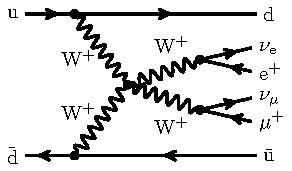
\includegraphics[width=0.30\linewidth]{feynman/LO_EW_5}
          \raisebox{.5ex}{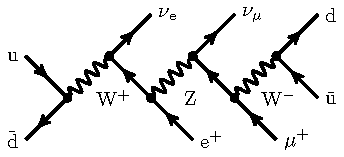
\includegraphics[width=0.35\linewidth]{feynman/LO_EW_2}}
          \raisebox{-1.8ex}{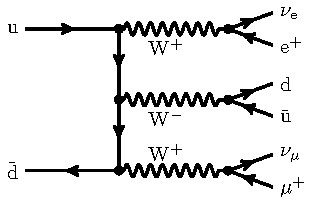
\includegraphics[width=0.32\linewidth]{feynman/LO_EW_3}}
\end{center}
        \caption{Sample tree-level diagrams that contribute to the process $\Pp\Pp\to\mu^+\nu_\mu\Pe^+\nu_{\Pe}\Pj\Pj$ at order $\mathcal{O}{\left(\alpha^{6}\right)}$.
        In addition to typical VBS contributions (left), this order also possesses $s$-channel contributions such as decay chain (middle) and tri-boson contributions (right).}
\label{diag:LO}
\end{figure*}

The scattering of two positively-charged $\PW$ bosons with their subsequent decay into different-flavour leptons 
can proceed at the LHC through the partonic process:
%
\begin{equation}
\Pp\Pp\to\mu^+\nu_\mu{\rm e}^+\nu_{\rm e}\,\Pj\Pj+\mathrm{X}.
\end{equation}

This process possesses three LO contributions of different orders.
At LO, this process can proceed via three different coupling-order combinations:
$\mathcal{O}{\left(\alpha^{6}\right)}$, $\mathcal{O}{\left(\alphas^{2}\alpha^{4}\right)}$, and $\mathcal{O}{\left(\alphas\alpha^{5}\right)}$.
The first, commonly referred to as EW contribution or VBS,\footnote{The name VBS is used even though not all Feynman diagrams involve the scattering
of vector bosons.} receives the contributions from Feynman diagrams such as those in Fig.~\ref{diag:LO}:
in addition to genuine VBS contributions (left diagram), it also features $s$-channel contributions with non-resonant vector bosons 
(center diagram) or from
triple-boson production (right diagram).
Note that $s$-, $t$-, and $u$-channel contributions are defined according to the quark lines.
$s$-channel denotes all Feynman diagrams where the two initial-state partons are connected by a continuous fermion line.
$u$-channel refers to contributions with crossed fermion lines with respect to $t$-channel, which appears for identical quarks or anti-quarks in the final state
The $s$-channel contributions will play a particular role in the study of the various contributions in Sec.~\ref{subsec:contributions}.

When using approximations, care must be taken that only gauge-invariant subsets are considered to obtain physically meaningful results. We will discuss the commonly-used possible choices in detail in the next section.

The second coupling combination corresponds to diagrams with a gluon connecting the two quark lines, and with the $\PW$ bosons 
radiated off the quark lines. Because of the different colour structure, this contribution features a 
different kinematic behaviour than VBS. Nonetheless they share the same final state, and this class of contributions therefore constitutes an irreducible background to the genuine VBS signal.

Finally, the third contribution is the interference of the two types of amplitudes described above.
It is non-zero only for those partonic subprocesses which involve identical quarks or antiquarks.
Such a contribution is typically small (3\%) within typical experimental cuts~\cite{Biedermann:2017bss}.

In experimental measurements, special cuts, called VBS cuts, are designed to enhance the EW contribution over the QCD one and to suppress the interference.
These cuts are based on the different kinematical behaviour of the contributions.
The EW contribution is characterised by two jets with large rapidities as well as a large invariant mass.
The two $\PW$ bosons are mostly produced centrally.
This is in contrast to the QCD contribution which favours jets in the central region.
Therefore, the event selection usually involves rapidity-difference and invariant-mass cuts for the jets.
Note that, as pointed out in Ref.~\cite{Biedermann:2017bss}, when considering full amplitudes, the separation between EW and QCD production becomes ill
defined.
Hence, combined measurements which are better theoretically defined should be preferably performed by the experimental collaborations at the LHC.